\documentclass[xcolor=dvipsnames,10pt]{beamer}

\usetheme[presnum=04]{u18fest}

\subtitle{Marco Bayesiano para el análisis de datos,\\
  calibración de parámetros y modelamiento inverso}
\title{Probabilidad conjunta\\
  y condicional}%
\institute{Universidad Industrial de Santander}%
\date{U18 Fest}

\usepackage{subcaption}
\usepackage{pgfplots}
\usetikzlibrary{positioning,calc}
\usetikzlibrary{external}
\tikzexternalize[export=false, prefix=04-figures/]
\captionsetup[subfigure]{labelformat=empty}

\begin{document}

\begin{frame}[noframenumbering]
  \titlepage
\end{frame}

\begin{frame}
  \frametitle{Resultados de un referendo en dos regiones}
  \begin{columns}
    \begin{column}{0.48\textwidth}
      \begin{figure}
        \centering
        \begin{tikzpicture}[x=1.5cm, y=1.5cm]
          \draw (0, 0) rectangle+(1, 1);%
          \draw (0, 1) rectangle+(1, 1);%
          \draw (1, 0) rectangle+(1, 1);%
          \draw (1, 1) rectangle+(1, 1);%
          \node [align=center] at (0.5, 0.5) {%
            {\only<1>{$C$}}%
            {\only<2->{$(1, 0)$}}%
            \\$0.4$};%
          \node [align=center] at (1.5, 0.5) {%
            {\only<1>{$D$}}%
            {\only<2->{$(0, 0)$}}%
            \\$0.3$};%
          \node [align=center] at (0.5, 1.5) {%
            {\only<1>{$A$}}%
            {\only<2->{$(1, 1)$}}%
            \\$0.2$};%
          \node [align=center] at (1.5, 1.5) {%
            {\only<1>{$B$}}%
            {\only<2->{$(0, 1)$}}%
            \\$0.1$};%
          \node [align=center] at (0.5, 2.5) {Gana\\%
            {\only<1>{$G_1$}}%
            {\only<2->{$Y_1 = 1$}}%
          };%
          \node [align=center] at (1.5, 2.5) {Pierde\\%
            {\only<1>{$P_1$}}%
            {\only<2->{$Y_1 = 0$}}%
          };%
          \node [align=center] at (-0.6, 0.5) {Pierde\\%
            {\only<1>{$P_2$}}%
            {\only<2->{$Y_2 = 0$}}%
          };%
          \node [align=center] at (-0.6, 1.5) {Gana\\%
            {\only<1>{$G_2$}}%
            {\only<2->{$Y_2 = 1$}}%
          };%
          \node [align=center] at (1, 3) {Región 1};%
          \node [align=center, rotate=90] at (-1.4, 1) {Región 2};%
        \end{tikzpicture}
      \end{figure}
    \end{column}
    \begin{column}{0.48\textwidth}
      \begin{overprint}
        \onslide<1>
        Podemos pensar en términos de eventos
        \begin{itemize}
        \item $P(G_1) = P(A) + P(C) = 0.6$
        \item $P(P_1) = P(B) + P(D) = 0.4$
        \item Etc.
        \end{itemize}
        \onslide<2>
        O podemos pensar en variables aleatorias
        \begin{itemize}
        \item $Y_1$: Resultado en la región 1
        \item $Y_2$: Resultado en la región 2
        \item Variable vectorial
          \begin{equation*}
            Y =
            \begin{bmatrix}
              Y_1\\Y_2
            \end{bmatrix}
          \end{equation*}
          equivalente a $Y = [Y_1, Y_2]^{\top}$
        \end{itemize}
        \onslide<3->
        Introducimos la \emph{pmf conjunta}
        \begin{align*}
          p_Y(y) &= p_{Y_1 Y_2}(y_1, y_2)\\
          &= P \left ( \{Y_1 = y_1 \} \cup \{Y_2 = y_2 \} \right)
        \end{align*}
        \begin{itemize}
        \item $p_{Y_1 Y_2}(1, 0) = 0.4$
        \item $p_{Y_1 Y_2}(0, 0) = 0.3$
        \item Etc.
        \end{itemize}
      \end{overprint}
    \end{column}
  \end{columns}
\end{frame}
%
\begin{frame}
  \frametitle{Probabilidad conjunta y marginal}
  Considérese las dos variables aleatorias
  \begin{equation*}
    X \colon \Omega \to C_X, \quad Y \colon \Omega \to C_Y
  \end{equation*}
  \begin{itemize}
  \item \textbf{pmf conjunta}
    \begin{equation*}
      p_{XY}(x, y) = P \left ( \{ X = x \} \cup \{Y = y\} \right )
    \end{equation*}
    \pause%
    La pmf conjunta completamente define la distribución de probabilidad de ambas variables aleatorias
    \pause
  \item \textbf{pmfs marginales}
    \begin{equation*}
      p_X (x) = \sum_{y \in C_Y} p_{XY}(x, y), \quad
      p_Y (y) = \sum_{x \in C_X} p_{XY}(x, y)
    \end{equation*}
  \end{itemize}
\end{frame}
%
\begin{frame}
  \frametitle{Resultados de un referendo en dos regiones}
  \begin{columns}
    \begin{column}{0.48\textwidth}
      \begin{figure}
        \centering
        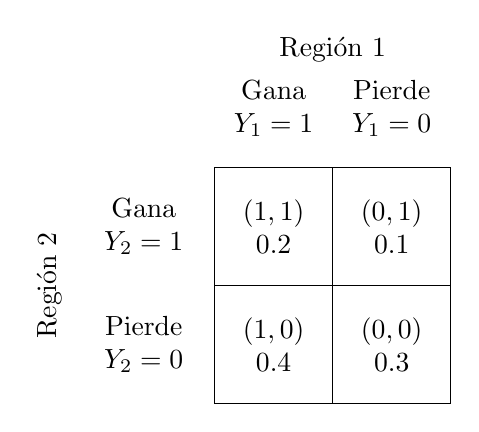
\begin{tikzpicture}[x=1.5cm, y=1.5cm]
          \draw (0, 0) rectangle+(1, 1);%
          \draw (0, 1) rectangle+(1, 1);%
          \draw (1, 0) rectangle+(1, 1);%
          \draw (1, 1) rectangle+(1, 1);%
          \node [align=center] at (0.5, 0.5) {%
            {{$(1, 0)$}}%
            \\$0.4$};%
          \node [align=center] at (1.5, 0.5) {%
            {{$(0, 0)$}}%
            \\$0.3$};%
          \node [align=center] at (0.5, 1.5) {%
            {{$(1, 1)$}}%
            \\$0.2$};%
          \node [align=center] at (1.5, 1.5) {%
            {{$(0, 1)$}}%
            \\$0.1$};%
          \node [align=center] at (0.5, 2.5) {Gana\\%
            {{$Y_1 = 1$}}%
          };%
          \node [align=center] at (1.5, 2.5) {Pierde\\%
            {{$Y_1 = 0$}}%
          };%
          \node [align=center] at (-0.6, 0.5) {Pierde\\%
            {{$Y_2 = 0$}}%
          };%
          \node [align=center] at (-0.6, 1.5) {Gana\\%
            {{$Y_2 = 1$}}%
          };%
          \node [align=center] at (1, 3) {Región 1};%
          \node [align=center, rotate=90] at (-1.4, 1) {Región 2};%
        \end{tikzpicture}
      \end{figure}
    \end{column}
    \begin{column}{0.48\textwidth}
      pmf marginal de $Y_1$
      \begin{gather*}
        \begin{aligned}
          p_{Y_1}(1) &= \sum_{y_2} p_{Y_1 Y_2}(1, y_2)\\
          &= p_{Y_1 Y_2}(1, 1) + p_{Y_1 Y_2}(1, 0)\\
          &= 0.2 + 0.4 = 0.6
        \end{aligned}\\
        \begin{aligned}
          p_{Y_1}(0) &= \sum_{y_2} p_{Y_1 Y_2}(0, y_2)\\
          &= p_{Y_1 Y_2}(0, 1) + p_{Y_1 Y_2}(0, 0)\\
          &= 0.1 + 0.3 = 0.4
        \end{aligned}
      \end{gather*}
    \end{column}
  \end{columns}
\end{frame}
%
\begin{frame}
  \frametitle{Independencia}
  Dos variables aleatorias son independientes si y sólo si
  \begin{equation*}
    p(x, y) = p(x) p(y) \ \text{ para todo } \ x \in C_X, \ y \in C_Y
  \end{equation*}
  i.e., si la pmf conjunta se factoriza en términos de las pmfs marginales
  \begin{itemize}
  \item Independencia implica que observar una variable aleatoria no provee información acerca del valor de la otra variable aleatoria
  \end{itemize}
\end{frame}
%
\begin{frame}
  \frametitle{Resultados de un referendo en dos regiones}
  \begin{columns}
    \begin{column}{0.48\textwidth}
      \begin{figure}
        \centering
        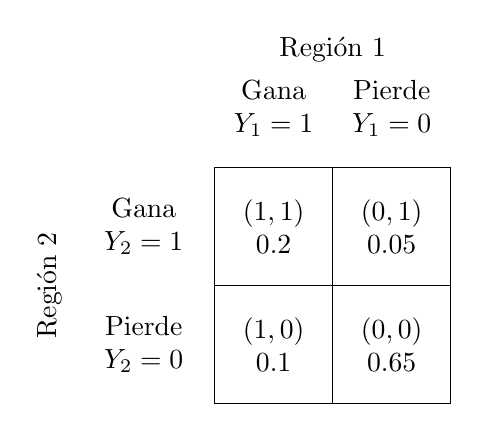
\begin{tikzpicture}[x=1.5cm, y=1.5cm]
          \draw (0, 0) rectangle+(1, 1);%
          \draw (0, 1) rectangle+(1, 1);%
          \draw (1, 0) rectangle+(1, 1);%
          \draw (1, 1) rectangle+(1, 1);%
          \node [align=center] at (0.5, 0.5) {%
            {{$(1, 0)$}}%
            \\$0.1$};%
          \node [align=center] at (1.5, 0.5) {%
            {{$(0, 0)$}}%
            \\$0.65$};%
          \node [align=center] at (0.5, 1.5) {%
            {{$(1, 1)$}}%
            \\$0.2$};%
          \node [align=center] at (1.5, 1.5) {%
            {{$(0, 1)$}}%
            \\$0.05$};%
          \node [align=center] at (0.5, 2.5) {Gana\\%
            {{$Y_1 = 1$}}%
          };%
          \node [align=center] at (1.5, 2.5) {Pierde\\%
            {{$Y_1 = 0$}}%
          };%
          \node [align=center] at (-0.6, 0.5) {Pierde\\%
            {{$Y_2 = 0$}}%
          };%
          \node [align=center] at (-0.6, 1.5) {Gana\\%
            {{$Y_2 = 1$}}%
          };%
          \node [align=center] at (1, 3) {Región 1};%
          \node [align=center, rotate=90] at (-1.4, 1) {Región 2};%
        \end{tikzpicture}
      \end{figure}
    \end{column}
    \begin{column}{0.48\textwidth}
      \begin{itemize}
      \item $p_{Y_1}(1) = 0.3$
      \item $p_{Y_2}(1) = 0.25$
      \item $p_{Y_1 Y_2}(1, 1) = 0.2 \neq 0.3 \times 0.25$
      \end{itemize}
      ... por lo tanto, $Y_1$ y $Y_2$ \textbf{no} son independientes
    \end{column}
  \end{columns}
\end{frame}
%
\begin{frame}
  \frametitle{Probabilidad condicional}
  Introducimos la \emph{pmf condicional} $p_{X \mid Y}(x \mid y)$
  \begin{itemize}
  \item Indica la probabilidad de $X = x$ dado que se ha observado que $Y = y$
  \item Relacionada con la pmf conjunta y las pmfs marginales a través de la relación
    \begin{equation*}
      p_{XY}(x, y) = p_{X \mid Y}(x \mid y) p_Y(y)
    \end{equation*}
  \item Naturalmente,
    \begin{equation*}
      p_{XY}(x, y) = p_{Y \mid X} (y \mid x) p_X(x)
    \end{equation*}
  \end{itemize}
\end{frame}
%

\begin{frame}
  \frametitle{Resultados de un referendo en dos regiones}
  \vskip1em
  \begin{columns}
    \begin{column}{0.48\textwidth}
      \begin{figure}
        \centering
        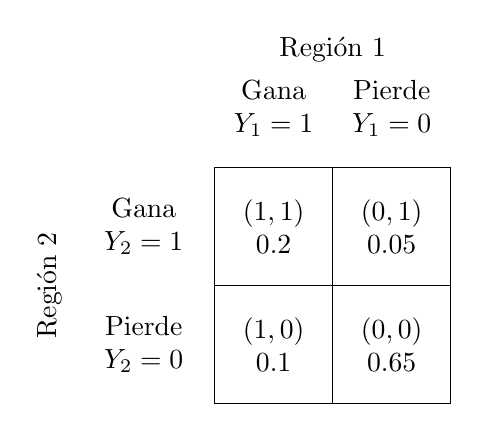
\begin{tikzpicture}[x=1.5cm, y=1.5cm]
          \draw (0, 0) rectangle+(1, 1);%
          \draw (0, 1) rectangle+(1, 1);%
          \draw (1, 0) rectangle+(1, 1);%
          \draw (1, 1) rectangle+(1, 1);%
          \node [align=center] at (0.5, 0.5) {%
            {{$(1, 0)$}}%
            \\$0.1$};%
          \node [align=center] at (1.5, 0.5) {%
            {{$(0, 0)$}}%
            \\$0.65$};%
          \node [align=center] at (0.5, 1.5) {%
            {{$(1, 1)$}}%
            \\$0.2$};%
          \node [align=center] at (1.5, 1.5) {%
            {{$(0, 1)$}}%
            \\$0.05$};%
          \node [align=center] at (0.5, 2.5) {Gana\\%
            {{$Y_1 = 1$}}%
          };%
          \node [align=center] at (1.5, 2.5) {Pierde\\%
            {{$Y_1 = 0$}}%
          };%
          \node [align=center] at (-0.6, 0.5) {Pierde\\%
            {{$Y_2 = 0$}}%
          };%
          \node [align=center] at (-0.6, 1.5) {Gana\\%
            {{$Y_2 = 1$}}%
          };%
          \node [align=center] at (1, 3) {Región 1};%
          \node [align=center, rotate=90] at (-1.4, 1) {Región 2};%
        \end{tikzpicture}
      \end{figure}
    \end{column}
    \begin{column}{0.48\textwidth}
      Se observa que el referendo \emph{gana} en la región 2. 
      Cuál es la probabilidad de ganar en la región 1?
      \begin{align*}
        p_{Y_1 \mid Y_2}(1 \mid 1) &= \frac{p_{Y_1 Y_2}(1, 1)}{p_{Y_2}(1)}\\
        &= \frac{0.2}{0.25} \approx 0.8
      \end{align*}
      \pause%
      Compárese:
      \begin{itemize}
      \item $p_{Y_1}(1) = 0.3$
      \item $p_{Y_1 \mid Y_2}(1 \mid 1) = 0.8$
      \end{itemize}
    \end{column}
  \end{columns}
  \pause
  \vskip2em
  Observar $Y_2$ provee información acerca de $Y_1$
\end{frame}
%
\begin{frame}
  \frametitle{Independencia}
  Para dos variables aleatorias independientes,
  \begin{equation*}
    p_{XY}(x, y) = p_X(x) p_Y(y)
  \end{equation*}
  Por lo tanto,
  \begin{equation*}
    p_{X \mid Y}(x \mid y) = \frac{p_{XY}(x, y)}{p_Y(y)} = \frac{p_X(x) p_Y(y)}{p_Y(y)} = p_X(x)
  \end{equation*}
  i.e, la probabilidad de $X = x$ es independiente del valor de $Y$
\end{frame}
%
\begin{frame}
  \frametitle{pdf conjunta}
  \emph{Ejemplo}: Variable aleatoria normal bivariante
  \vskip1em
  \begin{figure}
    \centering
    \begin{subfigure}{0.48\textwidth}
      \centering%
      {%
        \tikzsetnextfilename{bvn00s}
        \tikzset{external/export=true}
        \begin{tikzpicture}
          \begin{axis}[samples=50, width=6cm, xmin=-3, xmax=3, ymin=-3, ymax=3, point meta max=0.2]
            \addplot3 [surf, shader=interp, samples=50, domain=-3:3] {exp(-(x^2+y^2-2*0.0*x*y)/(2*(1-0.0^2)))/(2*pi*sqrt(1-0.0^2))};%
            \addplot3 [contour gnuplot={draw color=red, labels=false, levels={0.025, 0.05, 0.075, 0.1, 0.125, 0.15, 0.175}}, z filter/.code={\def\pgfmathresult{0.3}}] {exp(-(x^2+y^2-2*0.0*x*y)/(2*(1-0.0^2)))/(2*pi*sqrt(1-0.0^2))};
          \end{axis}
        \end{tikzpicture}
      }
      \caption{$\rho = 0.0$}
    \end{subfigure}g
    \begin{subfigure}{0.48\textwidth}
      \centering%
      {%
        \tikzsetnextfilename{bvn06s}
        \tikzset{external/export=true}
        \begin{tikzpicture}
          \begin{axis}[samples=50, width=6cm, xmin=-3, xmax=3, ymin=-3, ymax=3, point meta max=0.2]
            \addplot3 [surf, shader=interp, samples=50, domain=-3:3] {exp(-(x^2+y^2-2*0.6*x*y)/(2*(1-0.6^2)))/(2*pi*sqrt(1-0.6^2))};%
            \addplot3 [contour gnuplot={draw color=red, labels=false, levels={0.025, 0.05, 0.075, 0.1, 0.125, 0.15, 0.175}}, z filter/.code={\def\pgfmathresult{0.3}}] {exp(-(x^2+y^2-2*0.6*x*y)/(2*(1-0.6^2)))/(2*pi*sqrt(1-0.6^2))};
          \end{axis}
        \end{tikzpicture}
      }
      \caption{$\rho = 0.6$}
    \end{subfigure}
  \end{figure}
\end{frame}
%
% \begin{frame}
%   \frametitle{Ejemplo}
%   Variable aleatoria normal bivariante con $\rho = 0.6$
%   \begin{figure}
%     \centering%
%     {%
%       \tikzsetnextfilename{bvn06c}
%       \tikzset{external/export=true}
%       \begin{tikzpicture}
%         \begin{axis}[name=contour, height=5cm, width=5cm, ymin=-3, ymax=3, xmin=-3, xmax=3, view={0}{90}, axis equal, samples=200]
%           \addplot3 [contour gnuplot={labels=false, levels={0.05, 0.1, 0.2, 0.25, 0.3, 0.35}}, thick] {exp(-(x^2+y^2-2*0.6*x*y)/(2*(1-0.6^2)))/(2*pi*sqrt(1-0.6^2))};
%         \end{axis}
%         \begin{axis}[name=y1, height=3cm, width=5cm, ymin=0, xmin=-3, xmax=3, at={(contour.north)}, yshift=0.5cm, anchor=south, ytick={0.0, 0.2, 0.4}, xticklabels={,,}]
%           \addplot [samples=100, no markers, blue, thick] {exp(-(x^2)/2)/sqrt(2*pi)};%
%         \end{axis}
%         \begin{axis}[name=y2, height=5cm, width=3cm, xmin=0, ymin=-3, ymax=3, at={(contour.south east)}, xshift=0.5cm, anchor=south west, xtick={0.0, 0.2, 0.4}, yticklabels={,,}]
%           \addplot function [samples=100, parametric=true, no markers, blue, thick] {exp(-(t^2)/2)/sqrt(2*pi), t};%
%         \end{axis}
%       \end{tikzpicture}
%     }
%   \end{figure}
% \end{frame}
% %
% \begin{frame}
%   \frametitle{Ejemplo}
%   Variable aleatoria normal bivariante con $\rho = 0.9$
%   \begin{figure}
%     \centering%
%     {%
%       \tikzsetnextfilename{bvn09c}
%       \tikzset{external/export=true}
%       \begin{tikzpicture}
%         \begin{axis}[name=contour, height=5cm, width=5cm, ymin=-3, ymax=3, xmin=-3, xmax=3, view={0}{90}, axis equal, samples=200]
%           \addplot3 [contour gnuplot={labels=false, levels={0.05, 0.1, 0.2, 0.25, 0.3, 0.35}}, thick] {exp(-(x^2+y^2-2*0.9*x*y)/(2*(1-0.9^2)))/(2*pi*sqrt(1-0.9^2))};
%         \end{axis}
%         \begin{axis}[name=y1, height=3cm, width=5cm, ymin=0, xmin=-3, xmax=3, at={(contour.north)}, yshift=0.5cm, anchor=south, ytick={0.0, 0.2, 0.4}, xticklabels={,,}]
%           \addplot [samples=100, no markers, blue, thick] {exp(-(x^2)/2)/sqrt(2*pi)};%
%         \end{axis}
%         \begin{axis}[name=y2, height=5cm, width=3cm, xmin=0, ymin=-3, ymax=3, at={(contour.south east)}, xshift=0.5cm, anchor=south west, xtick={0.0, 0.2, 0.4}, yticklabels={,,}]
%           \addplot function [samples=100, parametric=true, no markers, blue, thick] {exp(-(t^2)/2)/sqrt(2*pi), t};%
%         \end{axis}
%       \end{tikzpicture}
%     }
%   \end{figure}
% \end{frame}

\end{document}

% Local Variables:
% TeX-master: t
% TeX-engine: luatex
% TeX-command-extra-options: "-shell-escape"
% ispell-local-dictionary: "es_CO"
% End:
